\documentclass{article}
\usepackage[utf8]{inputenc}
\usepackage{graphicx}
\usepackage{etoolbox}
\usepackage[normalem]{ulem}
\useunder{\uline}{\ul}{}
\graphicspath{ {Graphics/} }
\AtBeginEnvironment{quote}{\singlespacing\small}

\title{Solar Cell I-V Curve Investigation \\ Practice Assessment}
\author{Thomas Bass}
\begin{document}

\maketitle


\part{The Plan}

\section{Working Title}
\begin{quote}
the working title of the investigation
\end{quote}
An investigation to show the I-V Charachteristics of a Solar cell

\section{Aim}
\begin{quote}
the aim of the investigation
\end{quote}
This investigation will
\begin{enumerate}
  \item Investigate the change of potential difference and current as the external resistance changes
  \item Investigate this with different intensities
\end{enumerate}

\section{Reaserch}
As this invetigation is to find the I-V charachteristics of a solar cell, I found an article explanining the predicted I-V Curves of solar cells. The article explains the general shape of an I-V Curve of a solar cell, which can be approximated by a reflected log curve, as seen in the graphic below:

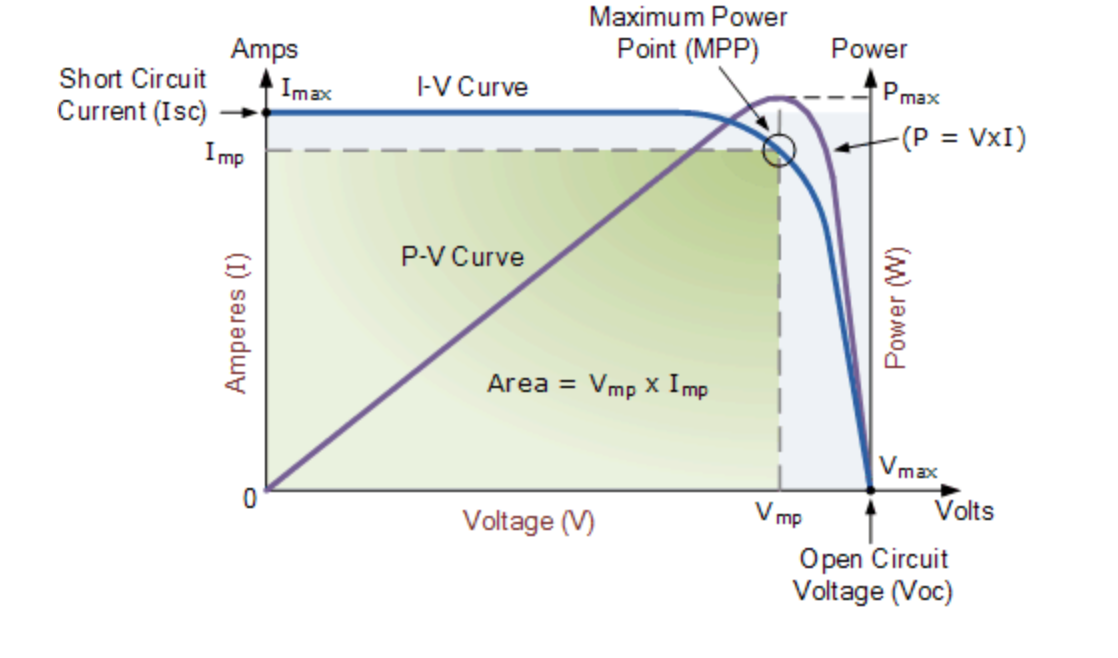
\includegraphics[scale=0.6]{imageone}

This graph also shows the Maximum Power Point, when the Current and Volatage are at their maximum, so the power is at the maximum, as $P=IV$
We will hopefully be able to comapre this graph to our actual results from the experiment.

\section{Initial Experiments}
\begin{quote}
an outline of the initial experiments
\end{quote}
For ease of recording, we want the apparatus to return values that can be accurately and quickly recorded. This means we want the equiptment to return values between 0 and 999, and no more than two decimal places
\begin{itemize}
  \item Find appropate sensitivity settings for the ammeter and voltmeter
  \begin{itemize}
    \item First, the solar cell was set up on a clamp stand, and the circuit constructed
    \item Then, the lamp was turned on and the light meter placed next to the solar cell
    \item The resistor was then closed to its lowest resistance, and the voltmeter sensitivity was set to the correct level. The lowest resistance will result in the highest voltage, so we set the voltmeter so that the greatest value of resistsance is not more than the sensitivity level is capable of showing
    \item The resistor was then opened to its greatest resistance, and the ammeter sensitivity was set in the same way as the voltmeter, as the highest resistance will reuslt in the highest current
  \end{itemize}
  \item Find appropriate variable resistors to use
  \begin{itemize}
    \item Once the Rheostat had been used, other potentiometers were provided
    \item To see if the range of resistance for these was appropate, each was connected to the current setup, and the maximum and minimum resistance was tested to see if the experiment could provide useful data with the sensitivity options provided by the multimeters
    \item The 100\Omega and 400\Omega variable resistors were rejected as they would not provide useful results, but the 50\Omega and 10\Omega variable resistors were used
  \end{itemize}

\end{itemize}
\subsection{Initial Experiment Results}
\begin{table}[!ht]
\centering
\caption{Initial Experiment Results}
\label{Initial Experiment Results}
\begin{tabular}{|l|l|l|}
\hline
\textbf{Resistor Setting} & \textbf{Potential Difference} & \textbf{Current} \\ \hline
Open (minimum)            & 105.0                         & 123              \\ \hline
Closed (maximum)          & 0.0                           & 442              \\ \hline
\end{tabular}
\end{table}
These results show that the sensitivity settings are correct, as the maximum results are within the range of the multimeter, and give results to a suitable decimal place.


\section{Apparatus}
\begin{quote}
a list of the required apparatus
\end{quote}
\begin{enumerate}
  \item Solar Cell
  \item Clamp stand
  \item 2x Multimeters for Voltmeter and Ammeter
  \item Desk lamp
  \item Light Meter
  \item Crorodile clips and cables
  \item Rheostat and Potentiometers
\end{enumerate}

%   TODO
\section{Initial Diagram}
\begin{quote}
a diagram of the initial experiment
\end{quote}

%   TODO
\section{Risk Assessment}
\begin{quote}
a risk assessment
\end{quote}

%   TODO
\section{Timeline}
\begin{quote}
a rough breakdown of how the two-week period of intensive practical work will be spent
\end{quote}
\pagebreak [4]
\part{The Report}

\section{Aim}
\begin{quote}
  a statement of aim
\end{quote}
This investigation will
\begin{enumerate}
  \item Investigate the change of potential difference and current as the external resistance changes
  \item Investigate this with different intensities
\end{enumerate}

\section{Results}

\begin{table}[!ht]
\centering
\caption{Measuring change in Potential Difference and Current with change in Light Level}
\label{my-label}
\begin{tabular}{|l|l|l|l|l|l|l|l|}
\cline{1-2} \cline{4-5} \cline{7-8}
\multicolumn{2}{|l|}{\textbf{320,000 Lux}} & {\ul }          & \multicolumn{2}{l|}{\textbf{120,000 Lux}}  & {\ul }          & \multicolumn{2}{l|}{\textbf{50,000 Lux}}   \\ \cline{1-2} \cline{4-5} \cline{7-8}
{\ul \textbf{Current}} & {\ul \textbf{PD}} & {\ul \textbf{}} & {\ul \textbf{Current}} & {\ul \textbf{PD}} & {\ul \textbf{}} & {\ul \textbf{Current}} & {\ul \textbf{PD}} \\ \cline{1-2} \cline{4-5} \cline{7-8}
\textit{200m}          & \textit{2}        & \textit{}       & \textit{200m}          & \textit{2}        & \textit{}       & \textit{200m}          & \textit{2}        \\ \cline{1-2} \cline{4-5} \cline{7-8}
114                    & 133               &                 & 54.3                   & 62                &                 & 24.2                   & 28                \\ \cline{1-2} \cline{4-5} \cline{7-8}
110                    & 198               &                 & 52.7                   & 234               &                 & 24                     & 43                \\ \cline{1-2} \cline{4-5} \cline{7-8}
105                    & 123               &                 & 48.1                   & 340               &                 & 23.9                   & 145               \\ \cline{1-2} \cline{4-5} \cline{7-8}
100                    & 291               &                 & 41.2                   & 395               &                 & 23.4                   & 211               \\ \cline{1-2} \cline{4-5} \cline{7-8}
90                     & 336               &                 & 35.2                   & 423               &                 & 22.7                   & 262               \\ \cline{1-2} \cline{4-5} \cline{7-8}
80                     & 364               &                 & 30.9                   & 437               &                 & 21.8                   & 298               \\ \cline{1-2} \cline{4-5} \cline{7-8}
70                     & 386               &                 & 28.3                   & 444               &                 & 21                     & 320               \\ \cline{1-2} \cline{4-5} \cline{7-8}
60                     & 406               &                 & 26.6                   & 448               &                 & 20.2                   & 338               \\ \cline{1-2} \cline{4-5} \cline{7-8}
50                     & 419               &                 & 25.4                   & 451               &                 & 19.7                   & 350               \\ \cline{1-2} \cline{4-5} \cline{7-8}
40                     & 433               &                 & 0                      & 495               &                 & 0                      & 473               \\ \cline{1-2} \cline{4-5} \cline{7-8}
30                     & 444               &                 &                        &                   &                 &                        &                   \\ \cline{1-2} \cline{4-5} \cline{7-8}
25.3                   & 449               &                 &                        &                   &                 &                        &                   \\ \cline{1-2} \cline{4-5} \cline{7-8}
0                      & 451               &                 &                        &                   &                 &                        &                   \\ \cline{1-2} \cline{4-5} \cline{7-8}
\end{tabular}
\end{table}
\\
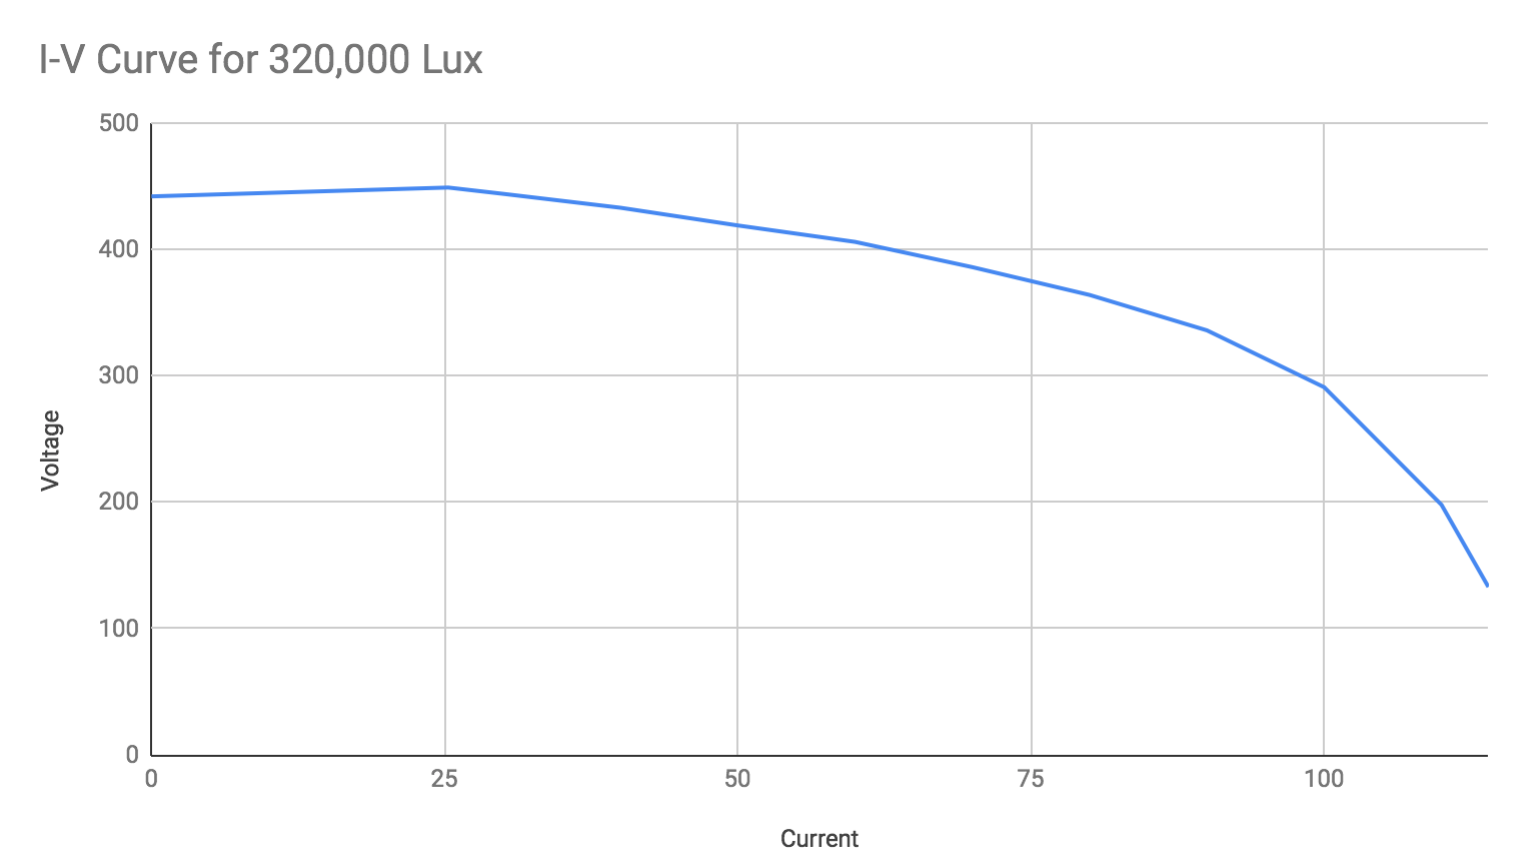
\includegraphics[scale=0.3]{ivcurve1}
\\
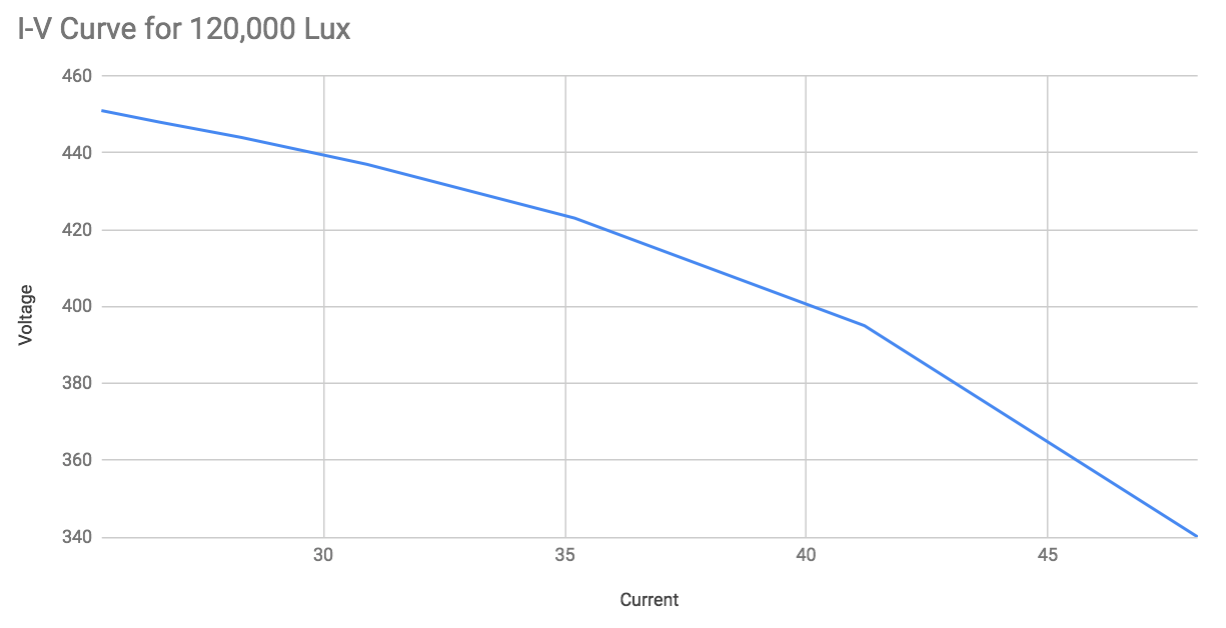
\includegraphics[scale=0.4]{ivcurve2}
\\
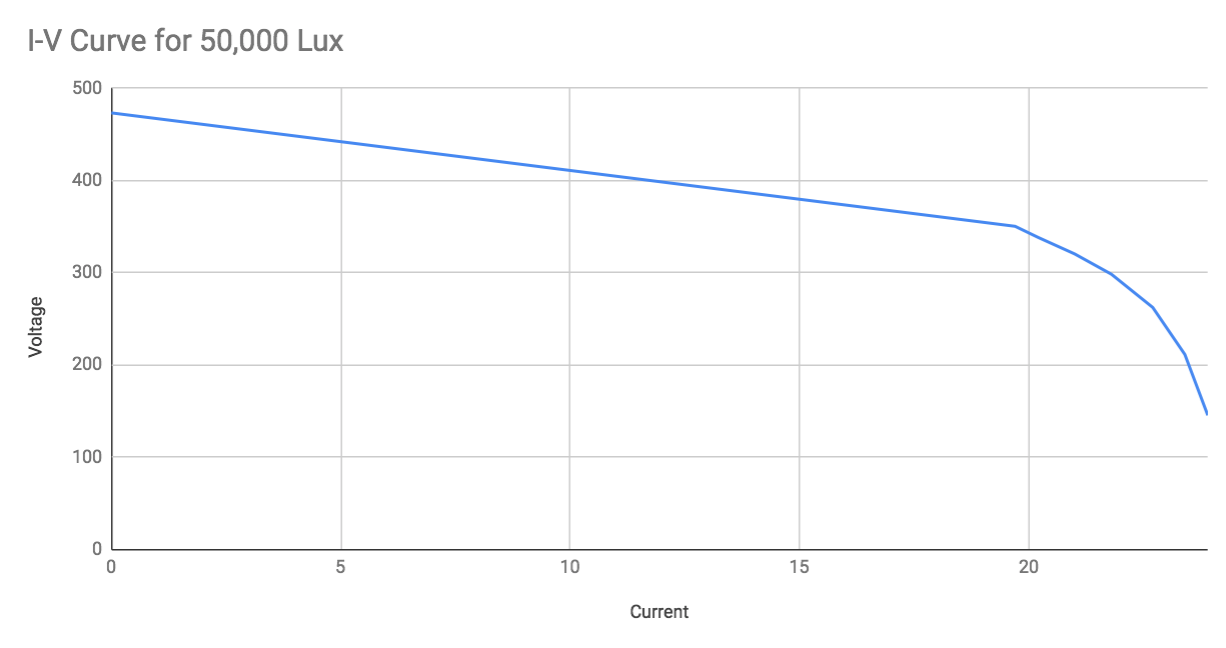
\includegraphics[scale=0.4]{ivcurve3}

\section{Summary}
\begin{quote}
  a word-processed summary of approximately 300 words written after completing the project, including an outline of any changes from the original plan
\end{quote}


From these results, we can see that each of the curves roughly approximate the predicted I-V curve. The charachteristic curve at 320,000 Lux shows many of the similar properties, with a plateau until 

\end{document}
